\section{От baseline к выбору архитектуры}

\subsection{001: baseline и первый beam search}
Первый реальный запуск BART 6+6/d512/FF2048 с LR $3\cdot10^{-4}$
проводился на Mac в FP32. Ранняя оценка времени составляла около шести
дней; далее отдельное обучение той же архитектуры перенесено на A100.
После одной сохранённой эпохи на 9\,463\,735 train получен
validation \loss{} 0.259714. Доступен checkpoint-147871;
последующая история после потери клиентского соединения не сохранилась.

На Test-001 greedy дал 6452/9929, то есть 64.98\% \pass{}.
Beam 4 на тех же весах и строках дал 6696/9929, или 67.44\%.
Он исправил 453 ответа и ухудшил 209: чистый выигрыш 244 решения
(+2.46 п.п.). Генерация 10\,000 ответов на A100 заняла
127.9 секунды для greedy и 167.8 секунды для beam 4.
Доля ошибок кода уменьшилась с 1.50\% до 0.72\%.

\textbf{Вывод.} Для этого checkpoint я увидел выигрыш от beam 4:
время выросло в 1.31 раза, но модель решила на 244 задачи больше.
Поэтому в следующих проверках я использовал beam 4.

\subsection{002: увеличение модели и диагностика срыва}
Модель увеличена до BART 8+8/d768/FF3072 и 139.25 млн параметров.
Одновременно train расширен до 98\% исходных данных, а global batch
увеличен с 64 до 128; обучение велось на двух A100 в BF16.
Это изменение всей конфигурации, а не изолированная проверка ширины.

Начальный LR $3\cdot10^{-4}$ привёл к неустойчивости:
лучший token loss 0.28247 получен на шаге 50\,000,
а после 50\,200 train loss резко вырос. Пять дальнейших validation
не улучшили минимум; early stopping завершил попытку на 75\,000.
Восстановлены лучшие веса шага 50\,000.

Для диагностики из одного checkpoint воспроизведены 600 шагов с
одинаковыми batch; использовались фиксированные 2048 validation-строки.
При исходном BF16/LR срыв повторился: максимальная норма градиента до
clipping составила 60.62, итоговый token loss --- 0.82960.
При делении LR на три получены 2.68 и 0.25433 соответственно.
FP32 с прежним LR дал 0.27448, но всплески градиентов сохранились.
На рисунке~\ref{fig:diagnostic} показан проверенный участок.

\begin{figure}[htbp]
\centering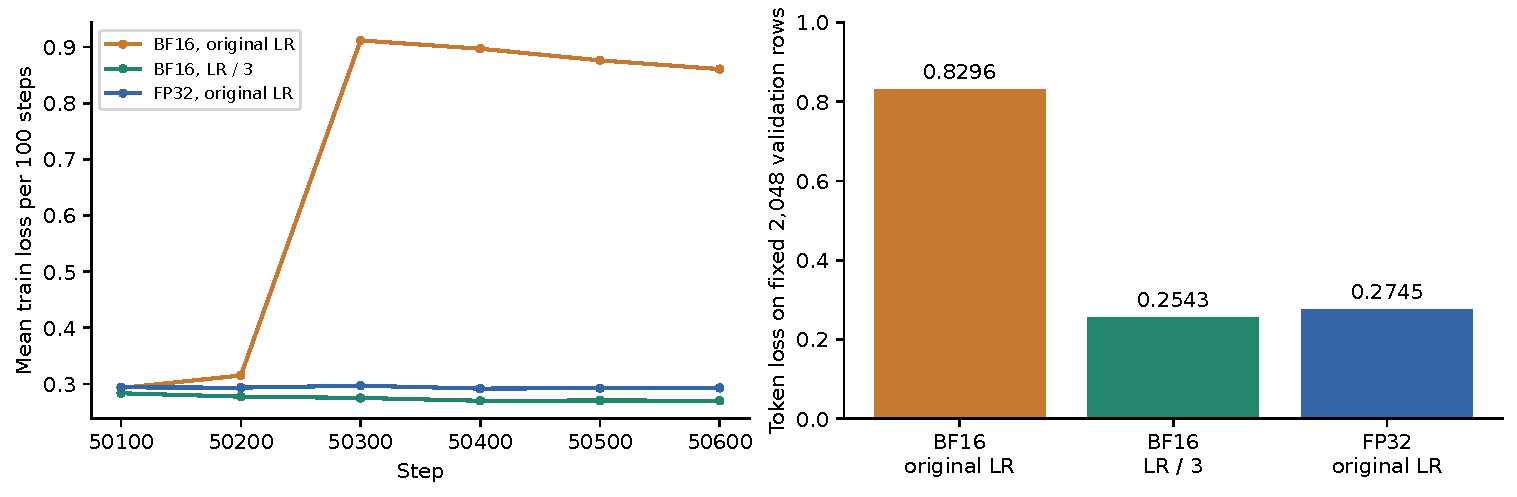
\includegraphics[width=\linewidth]{loss_diagnostic.pdf}
\caption{Диагностика модели 002. Слева --- средний train loss по 100 шагам,
справа --- token loss после 600 шагов на одной выборке 2048 примеров.
Эти короткие прогоны не доказывают долгосрочную устойчивость.}
\label{fig:diagnostic}
\end{figure}

Продолжение с checkpoint-50000 при LR $10^{-4}$ достигло суммарно
четырёх эпох и 362\,284 шагов. Лучший checkpoint-360000 имеет
validation token loss 0.1927033. На одном Test-002 последовательно
оценены checkpoint-50000, 90000 и 360000 (таблица~\ref{tab:old002}).

\begin{table}[htbp]
\centering\small\begin{tabular}{lrrr}
\toprule
Checkpoint & Greedy, \% & Beam 4, \% & Решено, beam 4 \\
\midrule
50000 & 60.21 & 63.03 & 6269/9946 \\
90000 & 68.09 & 69.69 & 6931/9946 \\
360000 & 71.66 & 72.84 & 7245/9946 \\
\bottomrule
\end{tabular}

\caption{Развитие модели 002 на неизменных 10\,000 строках Test-002,
9946 допустимых эталонов.}
\label{tab:old002}
\end{table}

\textbf{Вывод.} На диагностическом участке я смог устранить срыв,
уменьшив LR. После длительного продолжения я получил более высокое
качество генерации; финальный beam 4 добавил 118 решений к greedy
(+1.19 п.п.). После отправки этой модели в бота я получил
735/960 = 76.56\% на public. Это результат модели 002 на официальном
тесте, который я далее использовал для сравнения новых посылок.

\subsection{003: H100 и оптимизация цикла обучения}
Следующая конфигурация --- BART 10+10/d1024/FF4096, 303.18 млн
параметров, BF16, global batch 256 и LR $2\cdot10^{-4}$.
Исследовались расходы на padding, физический batch, fused AdamW
и \code{torch.compile}.
На коротком benchmark random/fused batch 128 дал около 614 примеров/с,
а группировка по длине и compile --- 1386 примеров/с;
padding уменьшился с 63.2\% до 25.5\%.
Начальная компиляция с прогревом заняла 96.3 секунды и исключена
из показателя throughput.

Дополнительный контроль на одинаковом checkpoint-7500, фиксированных
данных и трёх повторах сравнил attention (таблица~\ref{tab:attention}).
\begin{table}[htbp]
\centering\small
\begin{tabular}{llrr}
\toprule
Attention & Compile & Примеров/с, медиана & Пик allocated, ГиБ \\
\midrule
SDPA & нет & 1140.5 & 37.41 \\
FlashAttention-2 & нет & 1058.1 & 35.91 \\
FlashAttention-3 & нет & 1057.6 & 35.91 \\
SDPA & да & 1393.2 & 34.87 \\
FlashAttention-2 & да & 1041.7 & 33.44 \\
FlashAttention-3 & да & 1027.8 & 33.44 \\
\bottomrule
\end{tabular}
\caption{Training benchmark на H100: полный forward/backward/optimizer,
microbatch 128, accumulation 2, BF16.}
\label{tab:attention}
\end{table}

В штатном FA-адаптере обнаружено неверное применение encoder-маски
к decoder queries при unpadding cross-attention. В изолированном benchmark
адаптер исправлен и проверен по loss и градиентам; основной attention
не заменялся. Даже после этой проверки быстрее оказался SDPA с compile.
На свободной H100 batch 256 дал лишь +1.2\% throughput к 128$\times$2,
увеличив allocated memory с 34.87 до 65.79 ГиБ. Выбран 128$\times$2.

\textbf{Вывод.} Для своей модели с короткими последовательностями
я получил наибольшее ускорение от группировки по длине и SDPA+compile.
Их я оставил для продолжения поиска. Этот опыт показал мне, что
нужно измерять весь training pipeline: замена attention kernel сама
по себе не гарантирует ускорения. Здесь я сравнивал скорость обучения,
поэтому не использую эти числа как оценку качества генерации модели 003.

\subsection{004--005: глубина и learning rate на фиксированном бюджете}
Для быстрого отбора вместо полного обучения использован один миллион
фиксированных train, Val-20k, одна эпоха, global batch 256, seed 42,
warmup 5\% и cosine. BART-кандидаты различались глубиной и LR;
ширина оставалась 1024, FFN --- 4096.
В таблице~\ref{tab:h100} объединены восемь завершённых запусков двух серий.

\begin{table}[htbp]
\centering\small\begin{tabular}{lrrrr}
\toprule
E+D & LR & Парам., млн & Token loss & Время, с \\
\midrule
8+8 & 2e-04 & 244.39 & 0.394638 & 654.1 \\
8+12 & 2e-04 & 311.58 & 0.399215 & 828.0 \\
10+10 & 2e-04 & 303.18 & 0.436305 & 797.1 \\
10+10 & 1e-04 & 303.18 & 0.489001 & 796.1 \\
8+12 & 1e-04 & 311.58 & 0.496804 & 827.6 \\
12+8 & 1e-04 & 294.78 & 0.612622 & 764.1 \\
10+10 & 3e-04 & 303.18 & 0.850871 & 797.0 \\
12+8 & 2e-04 & 294.78 & 0.862528 & 762.7 \\
\bottomrule
\end{tabular}

\caption{Короткий поиск на H100: одинаковые 1M train и 20k validation.
Время --- wall time trial, а не время генерации.}
\label{tab:h100}
\end{table}

\begin{figure}[htbp]
\centering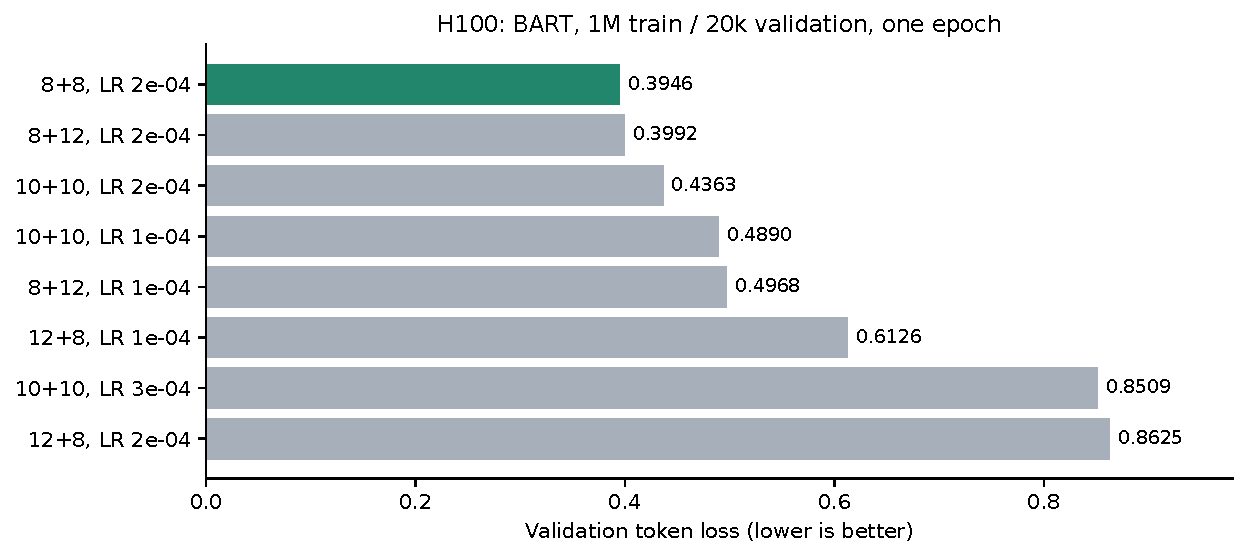
\includegraphics[width=.86\linewidth]{h100_sweep.pdf}
\caption{Validation token loss коротких BART-запусков. Меньшая модель
8+8 при LR $2\cdot10^{-4}$ оказалась лучшей в этом бюджете.}
\end{figure}

\textbf{Вывод.} Я не увидел преимущества более глубокого encoder 12+8.
Из проверенных вариантов я выбрал BART 8+8/d1024/FF4096
с LR $2\cdot10^{-4}$: он дал лучший loss при меньшем числе параметров
и меньшем времени. Я рассматривал это как отбор кандидата по раннему
обучению с одним seed, без вывода о превосходстве при любом бюджете.

\subsection{006--008: T5-style и копирование}
Проверена гипотеза, что другое устройство блоков или явное копирование
чисел из условия улучшат генерацию. Подготовленный H100-поиск T5
столкнулся с совместимостью TF32 API и Inductor; полноценным сравнимым
результатом T5 в этой части стали следующие завершённые Kaggle-запуски.
Отдельный smoke/preflight не рассматривается как измерение качества.

T5-style и Copy обучены на тех же 1M/20k, одну эпоху, LR
$2\cdot10^{-4}$, FP16, effective batch 256 на двух T4:
microbatch 16 на GPU, accumulation 8, gradient checkpointing.
Compile в окончательном Kaggle-рецепте отключён после исправления
ошибки runner, которая включала его через явно переданный backend.

\begin{table}[htbp]
\centering\small\begin{tabular}{lrrrr}
\toprule
Модель & Парам., млн & Token loss & Решено / 19886 & \pass{}, \% \\
\midrule
T5 & 247.31 & 1.012897 & 3333 & 16.7605 \\
Copy & 244.66 & 0.392547 & 10248 & 51.5337 \\
\bottomrule
\end{tabular}

\caption{Завершённые T5/Copy на Kaggle после одной эпохи.
Beam 4, 20\,000 validation, 19\,886 допустимых эталонов.}
\end{table}

Copy обучался около 2 ч 04 мин, T5 --- 2 ч 59 мин.
Генерация 20\,000 ответов на одной T4 для каждой модели заняла
1874.9 и около 4682.3 секунды соответственно.
\textbf{Вывод.} В этих настройках я получил у T5 заметно худший результат,
чем у Copy. Поэтому дальнейший отбор на A100 я сосредоточил на BART
и Copy. По одному LR, seed и одной эпохе я не делаю общего вывода
о возможностях T5. Скорость позднее обученного полного финалиста
я проверил отдельно на официальном тесте.

